% Chapter Template
\chapter{Discussion of survey results}

\label{chapter4}

\section{Summary of results}
In total, 31 responses were collected. The majority of respondents majored in law (58\%) vs non-law (42\%) respondents. Figure~\ref{fig:demo_1} and Figure~\ref{fig:demo_3} show the demographic data and responses relating to the respondents' beliefs regarding AI and data privacy. I originally intended to conduct analysis of the results across different demographics such as those with more expertise in computer science, or those who think that decisions by AI are not as useful. However, 31 respondents are insufficient for further meaningful demographic breakdown.

\begin{figure}[!ht]
  \centering
  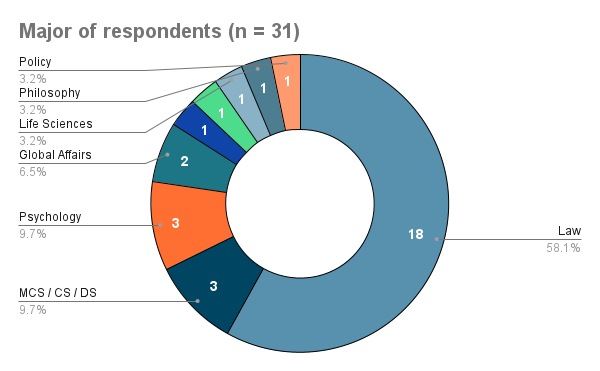
\includegraphics[width=0.85\linewidth]{figures/major_respondents.png}
  \caption{Breakdown of respondents' expertise by major}
  \label{fig:demo_1}
\end{figure}

% \begin{table}[!ht]
%     \resizebox{\textwidth}{!}{
%     \begin{tabular}{|p{0.45\linewidth}|l|l|}
%     \hline
%     \textbf{Major / Expected major}                    & \textbf{Count} & \textbf{Percentage of total (\%)} \\ \hline
%     Law                                                & 18             & 58                                \\ \hline
%     MCS / Computer Science / Data Science / Statistics & 3              & 9.7                               \\ \hline
%     Psychology                                         & 3              & 9.7                               \\ \hline
%     Global Affairs / Political Science                 & 2              & 6.5                               \\ \hline
%     Environmental Studies                              & 1              & 3.2                               \\ \hline
%     Economics                                          & 1              & 3.2                               \\ \hline
%     Life Sciences                                      & 1              & 3.2                               \\ \hline
%     Philosophy                                         & 1              & 3.2                               \\ \hline
%     Policy                                             & 1              & 3.2                               \\ \hline
%     \end{tabular}
%     }
%     \caption{Demographic breakdown of respondents according to academic discipline}
%     \label{tab:demo_1}
% \end{table}

\subsection{Part 1: Beliefs relating to AI \& data privacy}
Except for the questions relating to subject matter expertise (data privacy and AI), the level of agreement of law vs non-law respondents were about the same (Figure~\ref{fig:demo_3}). Law respondents had less expertise in AI, while conversely, non-law respondents had less experience with data privacy. Across all respondents, while they rated that decisions by AI could be a risk to society (about 4), they also agreed that decisions by AI could be equally useful. This perhaps suggests that the respondents think the balance between "usefulness" and "risks" are not zero-sum; AI could be very helpful in solving problems, but at the same time users should be cognisant of the risks.

\begin{figure}[!ht]
    \begin{subfigure}[b]{1\textwidth}
      \centering
      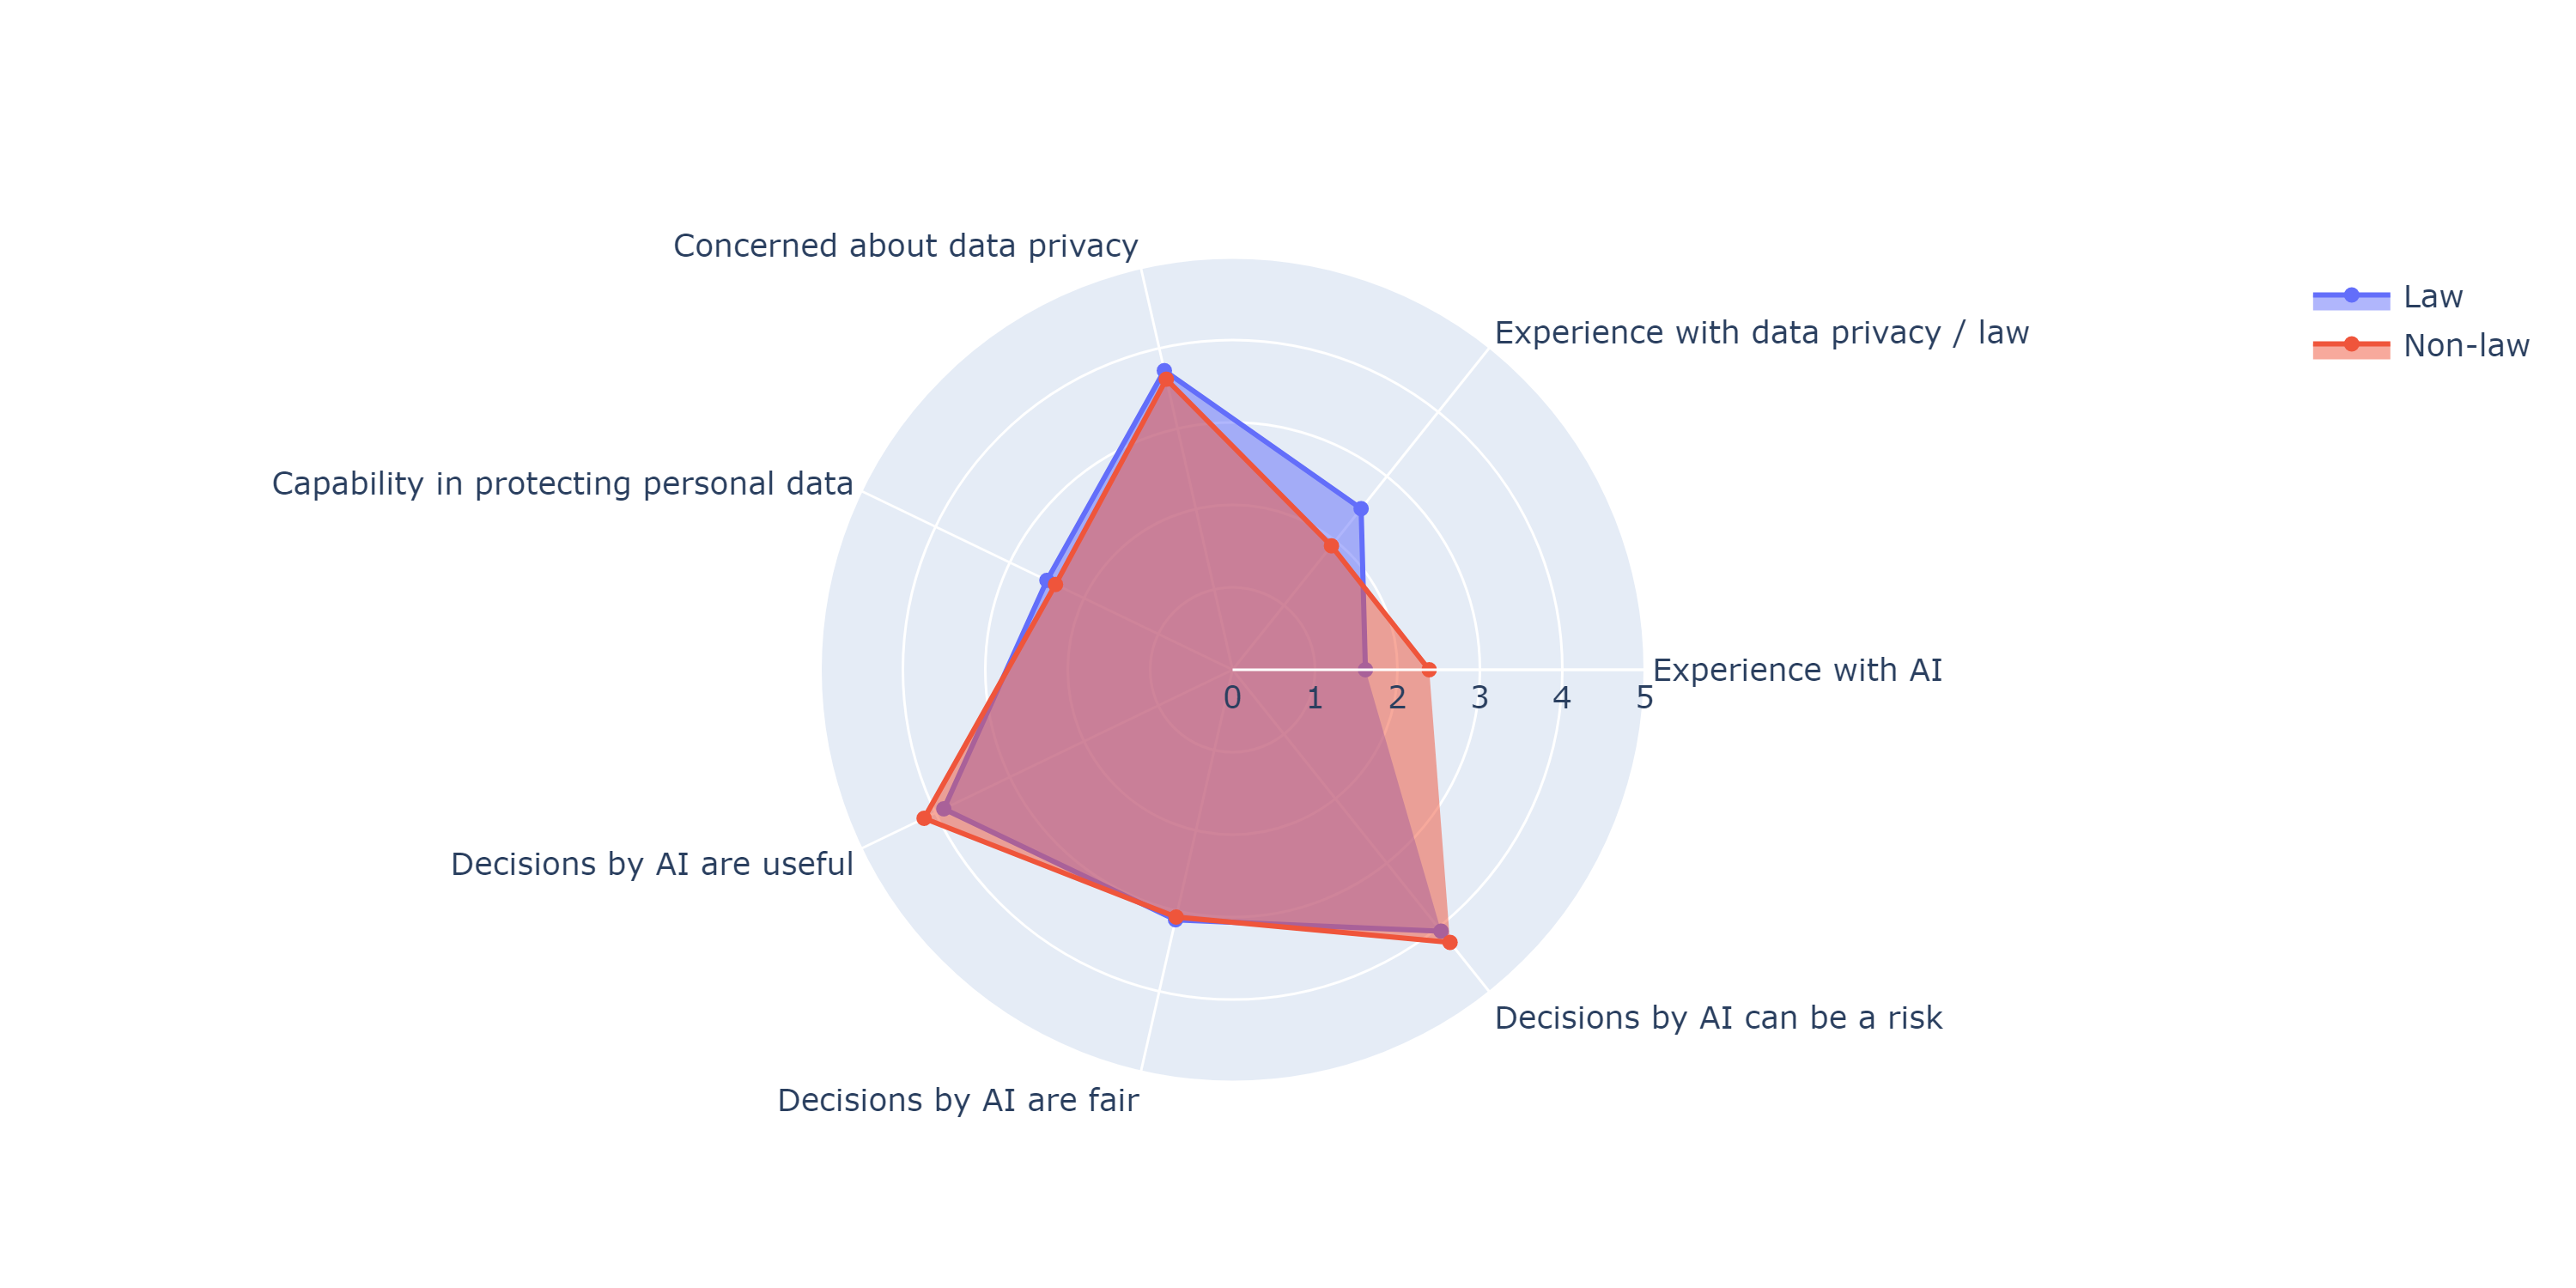
\includegraphics[width=1\linewidth]{figures/demo_3.png}
      \caption{Law vs Non-law respondents}
    \end{subfigure}
    \hfill
    \begin{subfigure}[b]{1\textwidth}
      \centering
      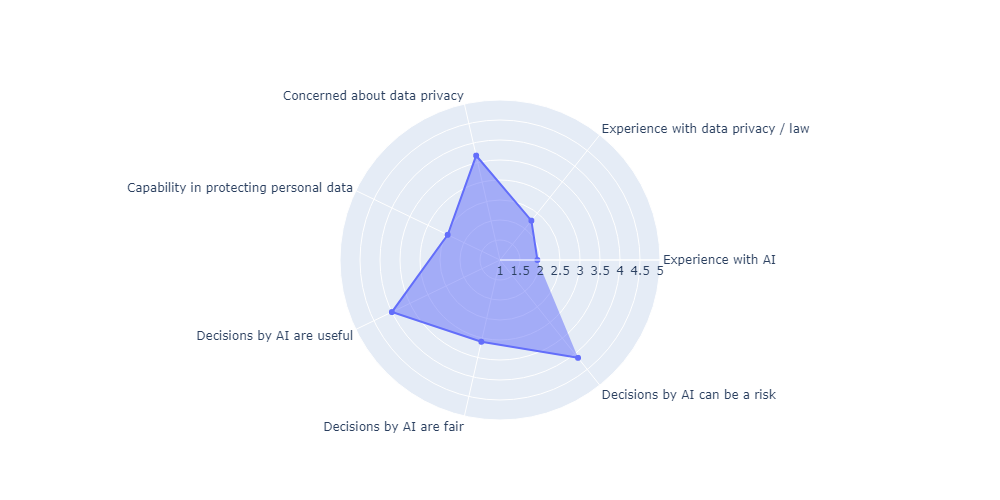
\includegraphics[width=1\linewidth]{figures/demo_4.png}
      \caption{All respondents}
    \end{subfigure}
    \caption{Mean scores of self-reported beliefs of respondents regarding AI \& data privacy. (1 = least agree, 5 = strongly agree. $n=31$)}
    \label{fig:demo_3}
\end{figure}

\subsection{Part 2 \& Part 6: Comparison of self-reported scores of explainability across the three contexts}
Using the Wilcoxon Rank Sum Test, I tested for the following, setting $\alpha = 0.1$: 
\begin{align*}
    H0&: \text{There is no increase / decrease in scores after viewing the explainations.} \\
    H1&: \text{There is an increase / decrease in scores after viewing the explainations.}
\end{align*}

The 1-sided test was used to check whether the distribution underlying the difference between the initial and final paired scores was symmetric below or above 0 (\cite{scipy}). Mathematically this difference can be stated as $d = i - f$, where $i$ and $f$ are the scores reported before and after viewing the explanations, and $d$ is the difference. Hence, if $d < 0$, then $i < f$ and the scores increased after viewing. Conversely, if $d > 0$, then $i > f$ and the scores decreased after viewing.

\begin{table}[!ht]
    \centering
    \resizebox{\textwidth}{!}{    
    \begin{tabular}{|p{0.3\textwidth}|p{0.15\textwidth}|p{0.15\textwidth}|p{0.15\textwidth}|p{0.15\textwidth}|p{0.15\textwidth}|p{0.15\textwidth}|}
    \hline
        \textbf{Question} & \textbf{Context 1: Increase} & \textbf{Context 1: Decrease} & \textbf{Context 2: Increase} & \textbf{Context 2: Decrease} & \textbf{Context 3: Increase} & \textbf{Context 3: Decrease} \\ \hline
        \textbf{Do you think model is effective?} & \cellcolor{red!25}0.013 & 0.987 & 0.932 & \cellcolor{red!25}0.0684 & 0.856 & 0.144 \\ \hline
        \textbf{Do you think model is a fair method?} & 0.382 & 0.618 & 0.841 & 0.159 & 0.933 & \cellcolor{red!25}0.0671 \\ \hline
        \textbf{Do you think model is a risk to society?} & 0.756 & 0.244 & 0.428 & 0.572 & 0.825 & 0.175 \\ \hline
        \textbf{Do you trust the prediction of the model?} & 0.887 & 0.113 & 0.945 & \cellcolor{red!25}0.055 & 0.837 & 0.163 \\ \hline
    \end{tabular}
    }
    \caption{p-values comparing whether there was a statistically significant increase / decrease in the explainability scores before and after viewing explanations.}
    \label{tab:context_comparison}
\end{table}

\begin{table}[!ht]
    \centering
    \begin{subtable}[h]{0.45\textwidth}
      \centering  
      \begin{tabular}{|l|l|}
        \hline
            \textbf{Context} & \textbf{p-value} \\ \hline
            1: Increase & 0.369 \\ \hline
            1: Decrease & 0.633 \\ \hline
            2: Increase & 0.940 \\ \hline
            2: Decrease & \cellcolor{red!25}0.060 \\ \hline
            3: Increase & 0.955 \\ \hline
            3: Decrease & \cellcolor{red!25}0.0450 \\ \hline
        \end{tabular}
        \caption{Mean scores by metrics}
        \label{tab:context_comparison_2a}
    \end{subtable}
    \hfill
    \begin{subtable}[h]{0.45\textwidth}
      \centering  
      \begin{tabular}{|l|l|}
            \hline  
            \textbf{Metric}                                    & \textbf{p-value}                     \\ 
            \hline
            Effective: Increase & 0.485  \\ \hline
            Effective: Decrease & 0.515  \\ \hline
            Fair: Increase      & 0.826  \\ \hline
            Fair: Decrease      & 0.174  \\ \hline
            Risk: Increase      & 0.660  \\ \hline
            Risk : Decrease     & 0.340  \\ \hline
            Trust: Increase     & 0.953  \\ \hline
            Trust: Decrease     & \cellcolor{red!25}0.0468 \\ \hline
        \end{tabular}
        \caption{Mean scores by contexts}
        \label{tab:context_comparison_2b}
    \end{subtable}
    \hfill
    \begin{subtable}[h]{0.45\textwidth}
      \centering
      \begin{tabular}{|l|l|}
        \hline
        \textbf{Increase} & \textbf{Decrease} \\ \hline
        0.844             & 0.156           \\ \hline
      \end{tabular}
    \caption{Mean scores across contexts and metrics}
    \end{subtable}
    \caption{p-values comparing mean scores}
    \label{tab:context_comparison_2}
\end{table}

The p-values of the tests are reported in Table~\ref{tab:context_comparison} ,~\ref{tab:context_comparison_2} and~\ref{tab:context_comparison_3}. For Table~\ref{tab:context_comparison_2a} and~\ref{tab:context_comparison_2b}, I took the mean of self-reported scores across contexts, and across each metric, respectively. "Increase" and "decrease" refer to the p-values of the 1-sided test that checks whether the scores significantly increased or decreased after viewing the explanations. For Table~\ref{tab:context_comparison_3}, the self-reported scores were averaged across both context and metric.  Here are the instances when $p<0.1$ (highlighted in red in the tables), and therefore $H0$ can be rejected in favour of $H1$ such that there was a statistically significant increase / decrease of scores after viewing the explanations:
\begin{enumerate}
    \item Effectiveness and trust significantly decreased for context 2 (PDPC), and fairness significantly decreased for context 3 (consumer). Only effectiveness significantly increased for context 1 (app developer) (Table~\ref{tab:context_comparison}). While trust technically did not have a statistically significant decrease for context 1, the p-value is quite close at 0.113. Hence, there seems to be an inverse relationship between effectiveness and trust for context 1, but a positive relationship for context 2.
    \item There is a statistically significant decrease in explainability metrics for context 1 and 2 when comparing the mean of the scores across the metrics (Table~\ref{tab:context_comparison_2a}) and for trust across the three contexts (Table~\ref{tab:context_comparison_2b}).
    \item The overall self-reported explainability when taking the mean of the scores across both contexts and metrics did not significantly increase / decrease (Table~\ref{tab:context_comparison_3}).
\end{enumerate}

Remember that the explanations given to respondents were deliberately chosen to demonstrate the limitations of the model. Hence, it can be inferred that respondents were more cognisant of such limitations when they answered the same questions again in Part 6. Here are some inferences that can be drawn from these observations:
\begin{enumerate}
    \item The inverse relationship between effectiveness and trust for context 1 (app developer) could be explained by the fact that respondents believed that software engineers may be more concerned with a standardised, consistent way to identify data practices, as someone who is not legally trained but is still subjected to data privacy obligations. Hence, self-reported effectiveness increased when they realised that the model would still do a better job at identifying data practices consistently compared to themselves. However, trust decreased because respondents also knew that the model could make wrong predictions. In this context, respondents were willing to bear some risk of getting predictions wrong in return for automated detection of data practices.
    \item For the positive relationship between effectiveness and trust for context 2 (PDPC), respondents were more concerned about retaining discretion in their decision making process. Since they knew that the model could make wrong predictions, combined with the fact that PDPC is the regulatory body that enforces data privacy, the costs of making a wrong decision is extremely high. Hence, even though the model is more "effective" since it is automated, it is not "effective" in terms of making a legally defensible decision given that it is fallible. Trust decreased because while the respondents believed that this model could make their jobs in identifying data breaches less repetitive (in that they would not have to read every data privacy policy manually), there is now a mismatch of expectations because respondents still have to ensure that the predictions given by the model are legally correct.
    \item For the consumer, as a person who is not trained in law or data science, they are subjected to how the app developer designed the app such that the app developer failed to disclose that the app was tracking cookies. However, as consumers are not legally trained, they cannot correct this breach of their privacy rights except by relying on the fallible predictions of the model. There is a chance that the model makes the wrong predictions, and the respondent fails to make a case to the PDPC. Therefore, it is not "fair" to the consumer that though their privacy was violated, they cannot do anything about it because of their reliance on the fallible model.
    \item Overall, a different weighting of these four values by the respondents can be inferred from the significance tests. The respondents were more concerned about having automated identification of data practices as a software engineer, over the risk of the model making a wrong prediction. In this case, effectiveness (in the sense of efficiency of identifying data practices) was prioritised above trust. This is contrasted with the PDPC context in which respondents were highly concerned of the risks of making a wrong decision more so than automating reading data privacy policies, and so fallible models are seen as impacting effectiveness and trust towards making sound legal decisions. The consumers are mainly concerned with their own interests and whether their rights would be vindicated, and so fallible models would greatly hinder them from pursuing this self-interest which is unfair for them.
    \item As to the comparison of aggregated scores in Table~\ref{tab:context_comparison_2a}, the fallibility of the model weighed heavily in the respondents' minds to reduce the explainability metrics in context 2 (PDPC) and context 3 (consumer). Perhaps the respondents thought that as app developers who were trained in programming, they would possess the requisite expertise to understand and work around the model's limitations compared to context 2 (PDPC) and context 3 (consumer) who may not have such technical knowledge and so are limited by the explanations that were presented to them.
    \item In the case of trust being the only metric that significantly decreased across the contexts, this perhaps shows the interrelation between of model transparency and trust. Intuitively, if respondents do not understand how a process works, they are less likely to trust the results of that process. However, since the respondents were made aware of the limitations of the model, they still have reduced trust not because they did not understand the model, but that their expectations of the model in producing objective, 100\% reliable predictions have been affected. Hence, there can be two plausible reasons for the loss in trust: the explanations were not effective in explaining the model, or that their expectations in the model have decreased as a result of being made aware of the limitations.
\end{enumerate}

\subsection{Part 3: Testing whether viewing more visualisations increase explainability}
\subsubsection{Analysis of the reported scores of "interpret" and "understand"}
There is a decreasing trend of both understanding and interpret after viewing each explanation, though understanding has a more negative gradient than interpret (Figure~\ref{fig:part3_trend}). It seems that respondents found the model less generally explainable after viewing more explanations, both in terms of the method of visualising the explanation (which is the "interpret" question), as well as understanding the inner logic of the model (the "understand" question). 

One interpretation of this decreasing trend suggests both the model and LIME were not very explainable. However, another interpretation could be that the respondents being more confused about how the model works globally after being exposed to specific predictions that were in themselves explainable, rather than being confused about a specific prediction of the model. As mentioned in Chapter~\ref{chapter2}, the visualisations for this part were specifically chosen to demonstrate the limits of the model by changing keywords which were strong predictors of the data practice. This means that respondents were being exposed to a more complex (and confusing) of the model globally as they found contradictions in how the model used certain keywords in some examples but not in others. Therefore, each explanation was actually effective in communicating to the respondents how that particular prediction was made, and therefore could be considered as locally explainable. However, as a whole, respondents' understandability of the model given the contradictions seen through comparing each explanation decreased. This decrease in explainability could be likened to a variation of the Dunning-Kruger effect (\cite{dunning_kruger}), whereby the respondents who initially had no experience with the model believed that they understood the model well because they were unaware of the complexity of the model, but when they were given more information, they had more awareness of the complexity and therefore reported a drop in explainability of the model as a whole. Therefore, LIME and the model could be said to be locally explainable, but globally not explainable. If this interpretation of the results is adopted, it would not be surprising since LIME is designed as a post-hoc, local XAI technique.

Another interpretation is that the underlying explainability method also influences the respondents' perception of the explainability of the visualisation technique (or vice versa). This can be seen by how there is a positive correlation between the understand and interpret scores. This is not surprising since if the visualisation technique is unclear or poor, explainability of the model itself would also decrease since respondents' only way of viewing the results of the explainability technique is through the visualisation technique. To respondents' both the visualisation technique and the explainability technique are one and the same thing.

\begin{figure}[!ht]
    \centering
    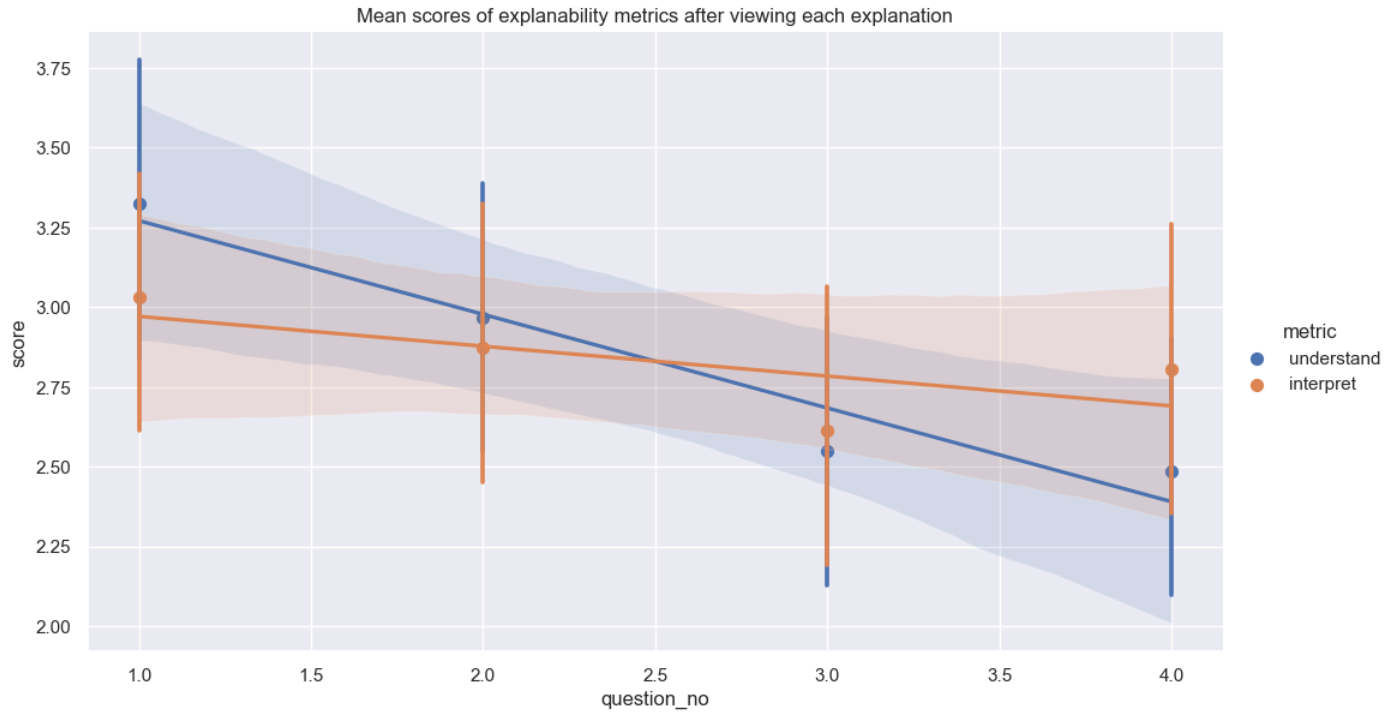
\includegraphics[width=1\linewidth]{figures/part3.png}
    \caption{Trend of the mean of self-reported understanding and interpretability after viewing each explanation}
    \label{fig:part3_trend}
\end{figure}

\subsubsection{Analysis of predicting counterfactuals}
It should be noted that the model itself gave quite ambivalent predicted probabilities for each data practice. For example, for the second counterfactual (Figure~\ref{fig:part3_counterfactuals_example_2}), the model predicted \texttt{Contact\_Email\_Address} at 25\% while \texttt{Identifier\_Cookie} was predicted at 23\%. Hence, the respondents' votes of predicting whether these counterfactuals would be classified as \texttt{Identifier\_Cookie} should also be roughly ambivalent if the respondents actually had a good sense of how the model would predict. Only the results of the first question had some similarity to the predicted probabilities of the model, while the results of the third question differed the most from the model (Figure~\ref{fig:part3_counterfactual}). Nevertheless, given the lack of any consistent trend across the questions, it is difficult to draw any definitive interpretations from the respondents' predictions of counterfactuals.

\begin{figure}[!ht]
    \begin{subfigure}[b]{1\textwidth}
      \centering
      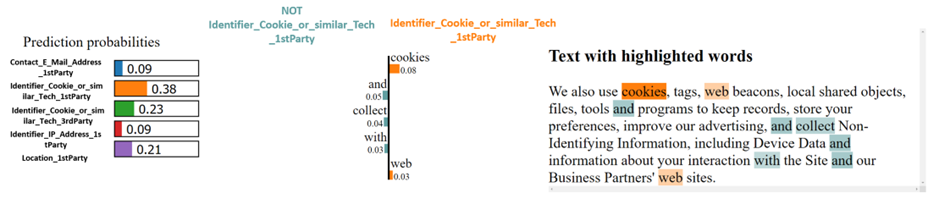
\includegraphics[width=1\linewidth]{figures/explanations_visualisations/counterfactual/3.2.png}
      \caption{Example explanation 1}
    \end{subfigure}
    \hfill
    \begin{subfigure}[b]{1\textwidth}
      \centering
      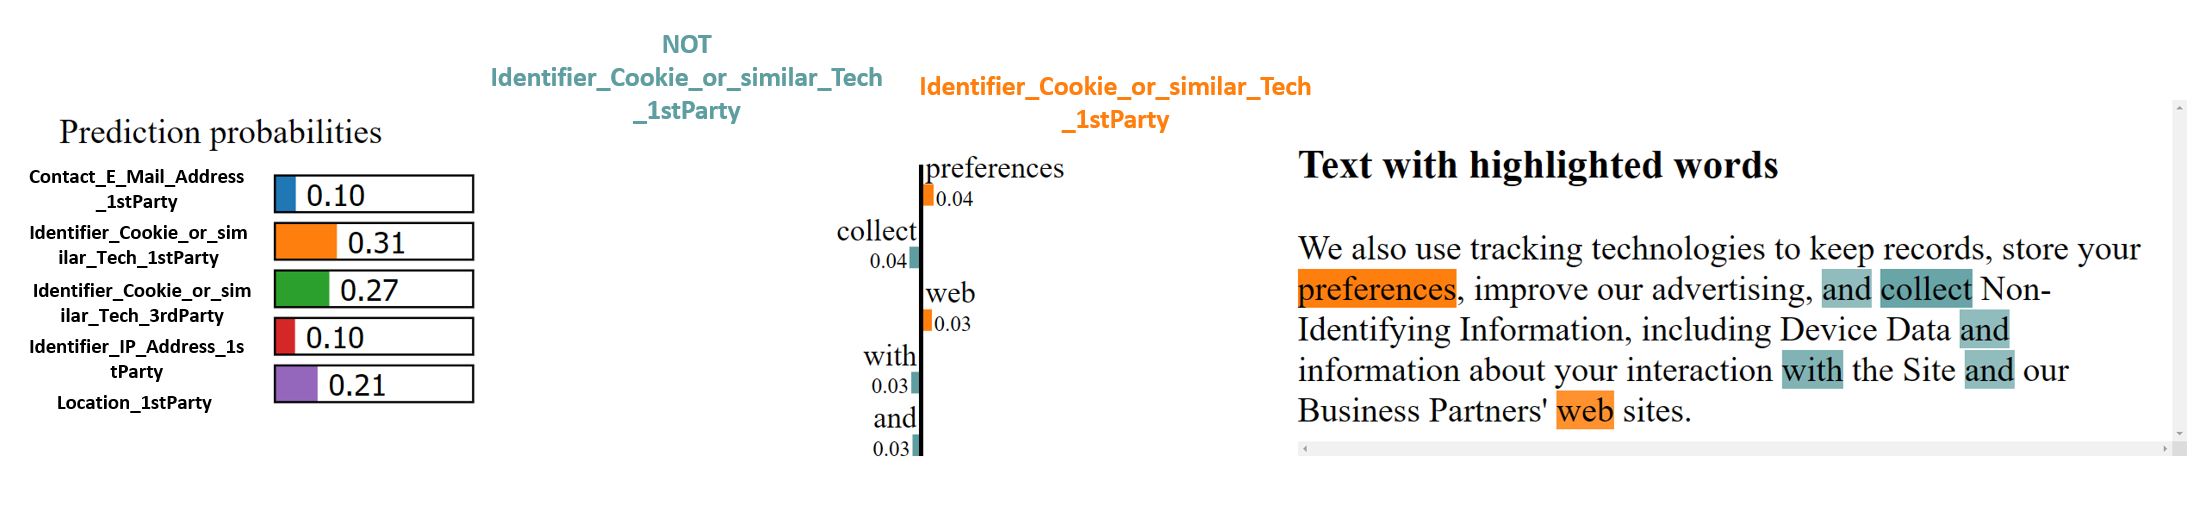
\includegraphics[width=1\linewidth]{figures/explanations_visualisations/counterfactual/3_2_counterfactual.png}
      \caption{Counterfactual explanation 1}
    \end{subfigure}
    \caption{Example and counterfactual explanation 1}
    \label{fig:part3_counterfactuals_example_1}
\end{figure}

\begin{figure}[!ht]
    \begin{subfigure}[b]{1\textwidth}
      \centering
      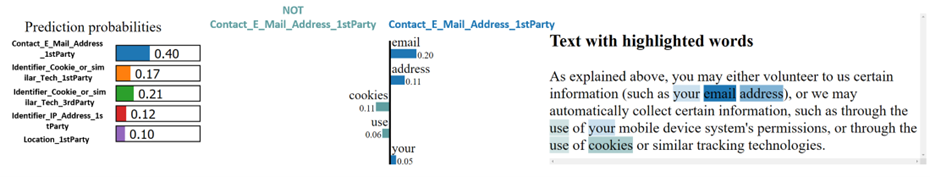
\includegraphics[width=1\linewidth]{figures/explanations_visualisations/counterfactual/3.3.png}
      \caption{Example explanation 2}
    \end{subfigure}
    \hfill
    \begin{subfigure}[b]{1\textwidth}
      \centering
      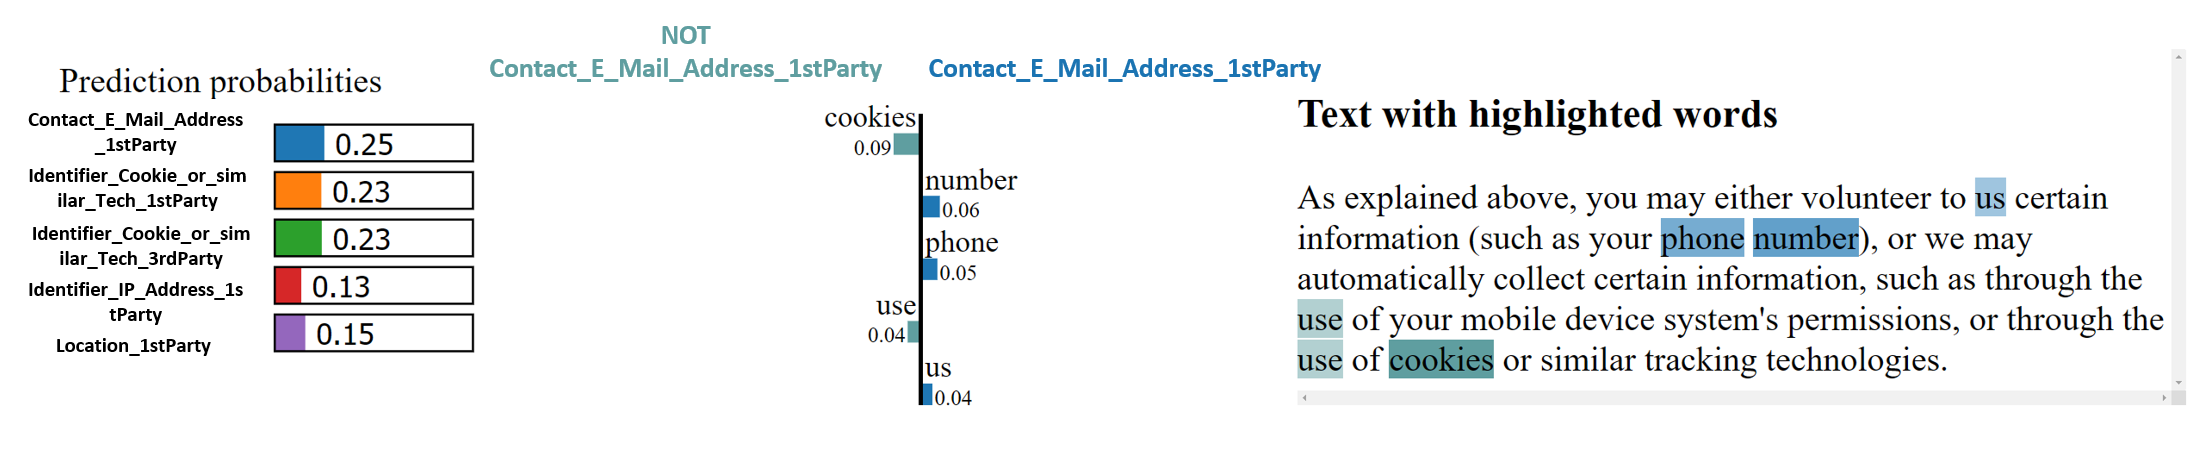
\includegraphics[width=1\linewidth]{figures/explanations_visualisations/counterfactual/3_3_counterfactual.png}
      \caption{Counterfactual explanation 2}
    \end{subfigure}
    \caption{Example and counterfactual explanation 2}
    \label{fig:part3_counterfactuals_example_2}
\end{figure}

\begin{figure}[!ht]
    \begin{subfigure}[b]{1\textwidth}
      \centering
      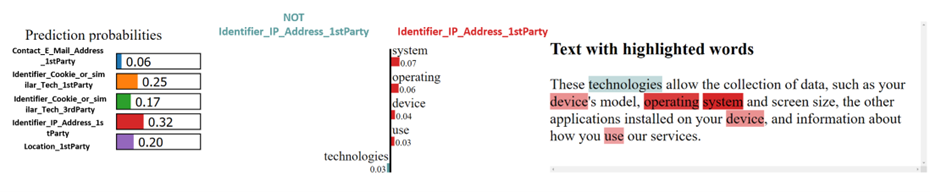
\includegraphics[width=1\linewidth]{figures/explanations_visualisations/counterfactual/3.4.png}
      \caption{Example explanation 3}
    \end{subfigure}
    \hfill
    \begin{subfigure}[b]{1\textwidth}
      \centering
      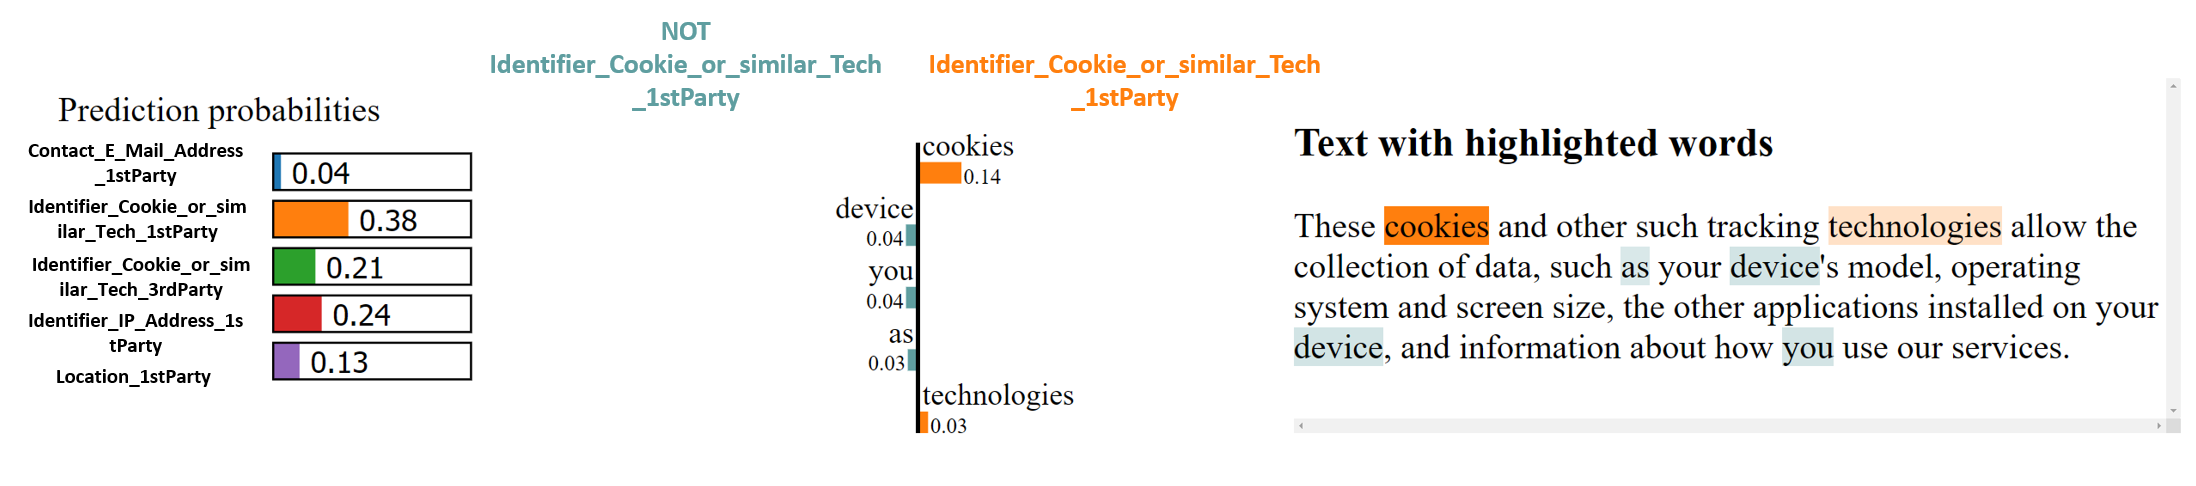
\includegraphics[width=1\linewidth]{figures/explanations_visualisations/counterfactual/3_4_counterfactual.png}
      \caption{Counterfactual explanation 3}
    \end{subfigure}
    \caption{Example and counterfactual explanation 3}
    \label{fig:part3_counterfactuals_example_3}
\end{figure}

\begin{figure}[!ht]
    \centering
    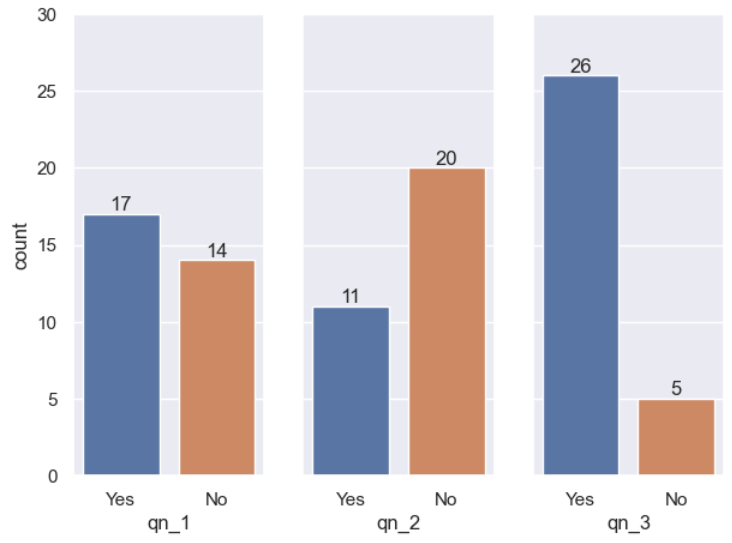
\includegraphics[width=1\linewidth]{figures/part_3_counterfactual.png}
    \caption{Votes for predicting whether counterfactual would be classified as \texttt{Identifier\_Cookie\_or\_Similar\_Tech\_1st\_Party}}
    \label{fig:part3_counterfactual}
\end{figure}

\subsection{Part 4 \& 5: Testing which model and word representation is more explainable}
As there were three questions in each section to test the explainability of each pair, the maximum total number of votes an option could get was $31 \times 3 = 93$. I totalled up the votes for each option for each part and each question in Figure~\ref{fig:part4} and~\ref{fig:part5}.

Overall, respondents found no difference in explainability between logistic regression and SVC (Figure~\ref{fig:part4}), while it was more contentious when comparing word representations, with a third split across the three options (Figure~\ref{fig:part5}). Remember that the model performance for each pair actually did not differ significantly, as mentioned in Chapter~\ref{chapter4}. In terms of comparing respondents' votes with the "ground truth" metric of model performance, we would expect most respondents to note that there are no differences between the explainabilty of the model. This was seen when comparing logistic regression vs SVC but not seen in the case of comparing Tf-IDF and GloVe. Votes for word representations had a higher spread of votes across the three options. While there is no majority consensus, the fact that the votes were almost equally split instead of being heavily weighted in favour of one category shows that respondents were more undecided in the explainability of the models. One inference of such results is that while respondents collectively did not give a definitive answer as to the more explainable word representation, there are still possible differences in explainability even when comparing models of relatively same performance, as picked up by the differences in distribution of the respondents' votes.

\begin{figure}[!ht]
    \begin{subfigure}[b]{0.75\textwidth}
      \centering
      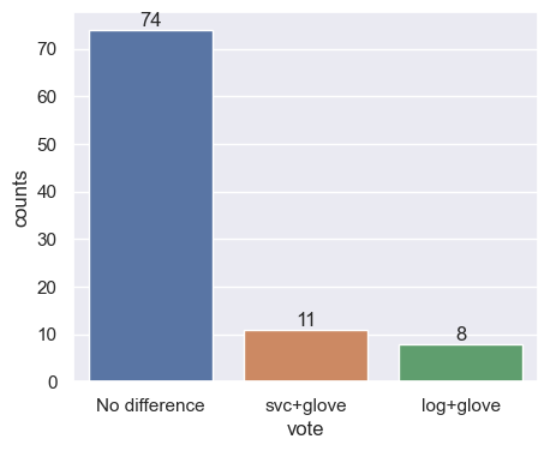
\includegraphics[width=1\linewidth]{figures/part4_votes.png}
      \caption{Total votes across 3 questions}
      %\label{fig:draketl}
    \end{subfigure}
    \hfill
    \begin{subfigure}[b]{1\textwidth}
      \centering
      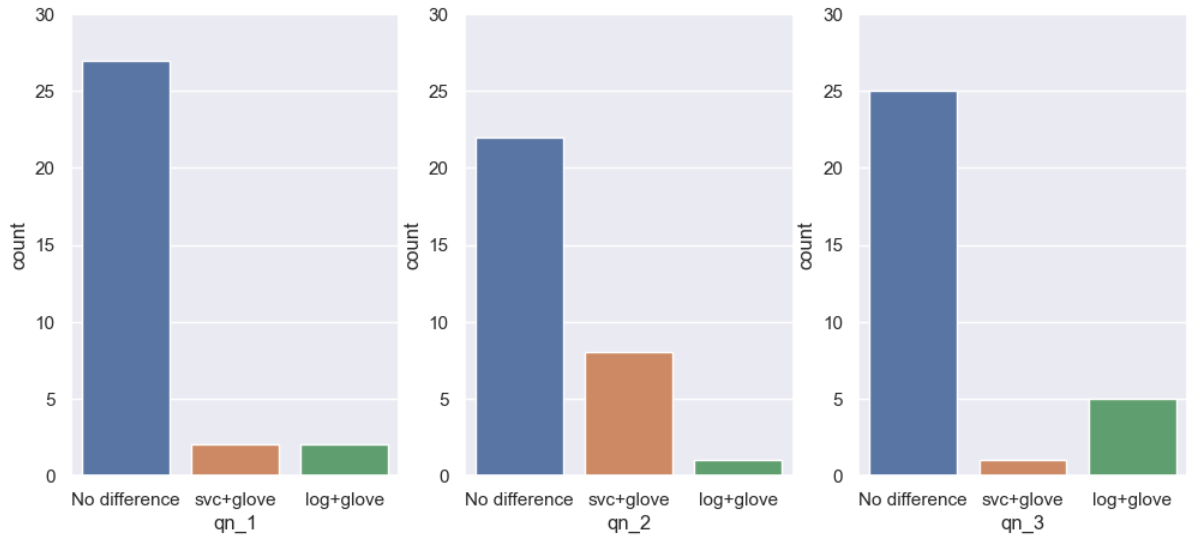
\includegraphics[width=1\linewidth]{figures/part_4_votes_1.png}
      \caption{Votes per question}
    \end{subfigure}
    \caption{Testing for which model was more explainable: Respondents' votes to whether SVC + GloVe or Logistic regression + GloVe were more explaninable}
    \label{fig:part4}
\end{figure}

\begin{figure}[!ht]
    \begin{subfigure}[b]{0.75\textwidth}
      \centering
      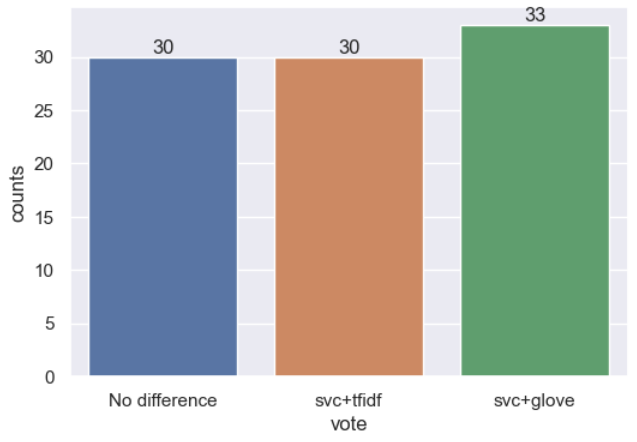
\includegraphics[width=1\linewidth]{figures/part5_votes.png}
      \caption{Total votes across 3 questions}
      %\label{fig:draketl}
    \end{subfigure}
    \hfill
    \begin{subfigure}[b]{1\textwidth}
      \centering
      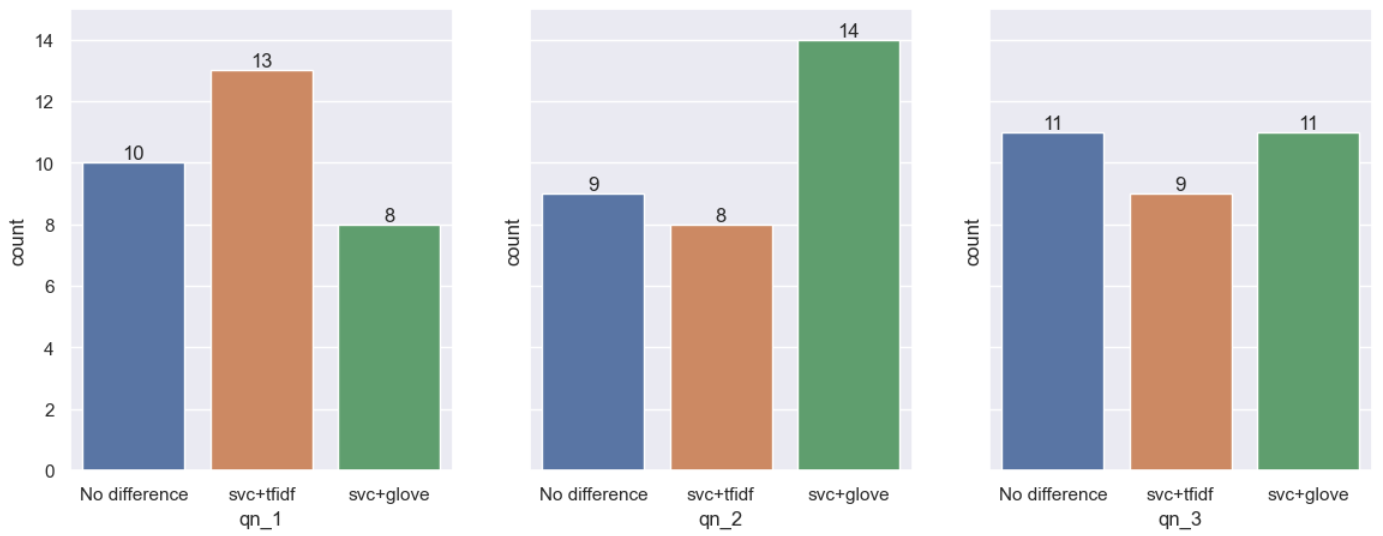
\includegraphics[width=1\linewidth]{figures/part_5_votes_1.png}
      \caption{Votes per question}
    \end{subfigure}
    \caption{Testing for which word representation was more explainable: Respondents' votes to whether SVC + TfIDF or SVC + GloVe were more explaninable}
    \label{fig:part5}
\end{figure}

\subsection{General discussion of results}
Here are some themes that arise from the preceding discussion:

\textit{Explainability is context sensitive.} 

Whether the self-reported explainability metrics significantly decreased or increased after viewing the explanations depended on the type of metric and the context. Respondents likely placed different emphasis on different values depending on the contexts, which resulted in differing evaluations of the the same explanation. While this finding is uncontroversial, it confirms current XAI research, and also demonstrates the complication of developing "more explainable" models when evaluating such explainability is context dependent, compared to typical metrics of performance such as precision / recall / F1. Further, perceptions of explainability can also be influenced by pre-existing expectations that users of models have. If users have the false conception that anything produced by a computer is "objective" and "trustworthy" without being aware that machine learning is inherently fallible, they are likely to report a reduction in explainability after viewing explanations that expose the fallibility of these models.

\textit{Global and local explainability should be evaluated in tandem.}

Global explanability can decrease even though local explanability may not be an issue. This is one of the limitations of local explainability techniques, as it allows users to understand the model through specific examples. Hence, explainability is highly dependent on the types and number of examples shown to users. If the examples chosen are insufficient or demonstrates an inuitively inconsistent pattern, users may be more confused about the model as a whole which affects global explainability. So it is important to consider global explanability by using different XAI techniques beyond just local explanations. Nevertheless, not all use cases require global explainability, such as perhaps the context of the consumer who may only be concerned with his own instance.

\textit{Models with similar performance metrics can have different perceptions of explainability.}

Different models and text representations can have different perceptions of explanability, such as the instance when Tf-IDF is compared against GloVe embeddings. While this finding might not surprising given that Tf-IDF is a purely count based metric that does not take into account word context unlike GloVe, such "explanability characteristics" of models can be taken into account when explanability is important for a particular use case beyond simply evaluating based on traditional performance metrics. Nevertheless, it is also important to note that the results obtained here are restricted to the particular dataset and implementation used, and I am not asserting that a particular model or text representation has an "intrinsic explainability quotient". 